\documentclass[12pt]{article}
\usepackage{xeCJK}
\usepackage{charter}
\usepackage{fullpage}
\usepackage[colorlinks=false]{hyperref}
\usepackage{ifthen}
\usepackage{comment}
\usepackage[title,titletoc]{appendix}
\usepackage{pagecolor}
\usepackage{amsmath}
\usepackage{amsfonts}
%\usepackage[normalem]{ulem}
\usepackage{siunitx}
\usepackage{amsthm}
\sisetup{per=slash, load=abbr}

\usepackage{pgfplots}
\usetikzlibrary{positioning}
\usetikzlibrary{fit}
\usetikzlibrary{snakes}
\usetikzlibrary{shapes.geometric}
\usetikzlibrary{patterns}
\usetikzlibrary{shapes,arrows,chains}
\usepgfplotslibrary{patchplots,colormaps}
\usetikzlibrary{calc}
\usetikzlibrary{positioning, fit}
\usetikzlibrary{backgrounds}
\usetikzlibrary{intersections}

\newcommand{\whitepaper}[1]{\begin{center}\fbox{\parbox{0.75\textwidth}{{\small
#1}}}\end{center}}

%\newcommand{\pcolor}{yellow!25}

\usepackage{setspace}
\usepackage{algorithm2e}
\bibliographystyle{ieeetr}

\usepackage{geometry}
\geometry{left=3cm,right=3cm,top=1.6cm,bottom=3cm,headheight=0pt,headsep=1.5em}
\usepackage{fancyhdr}
\pagestyle{fancy}
\chead{
\includegraphics[scale=0.2]{Nebulas.png}}  %在此处插入logo.pdf图片 图片靠左
\lhead{} % 页眉中间位置内容
\rhead{}
%\setlength{\topskip}{1em}


\usepackage{indentfirst}


\setCJKmainfont[BoldFont = STSongti-SC-Bold]{STSongti-SC-Regular}
\setCJKfamilyfont{hei}{SIL-Hei-Med-Jian}		%宋体
\setCJKfamilyfont{song}{SimSun}		%宋体
\setCJKfamilyfont{kai}{Kaiti}		%楷体
\setCJKfamilyfont{fang}{song}	%仿宋
\setCJKfamilyfont{li}{song}			%隶书
\setCJKfamilyfont{you}{Yuanti}		%幼圆

\newcommand{\song}{\CJKfamily{song}}	%宋体
\newcommand{\hei}{\CJKfamily{hei}}	%黑体
\newcommand{\kai}{\CJKfamily{kai}}	%楷体
\newcommand{\fs}{\CJKfamily{fang}}	%仿宋
\newcommand{\li}{\CJKfamily{li}}		%隶书
\newcommand{\you}{\CJKfamily{you}}	%幼圆
\newcommand{\reffig}[1]{图\ref{#1}}
\newcommand{\refsec}[1]{\S \ref{#1}}

\onehalfspacing   % ----------设置1.5倍行距(可能有意义,待调整)

\setlength{\parindent}{2.1em}
\setlength{\parskip}{0.3\baselineskip}
\newcommand{\nrcore}{Core Nebulas Rank}
\newcommand{\nrext}{Extended Nebulas Ranks}
\newcommand{\dom}{{\; \texttt{dom}\;}}

\setCJKsansfont[BoldFont = STHeitiSC-Medium]{STHeitiSC-Light}


\newtheorem{property}{特征}
%\addbibresource{reference.bib}

\begin{document}
\pagestyle{empty}
\renewcommand{\contentsname}{目录}
\renewcommand{\abstractname}{摘要}
\renewcommand{\refname}{参考文献}
%\renewcommand{\nomname}{术语表(按首字母排序)}
\renewcommand{\figurename}{图}
\renewcommand{\tablename}{表}
\renewcommand{\baselinestretch}{1.5}
\renewcommand{\appendixname}{附录}
\renewcommand{\proofname}{证明}


\begin{titlepage}
  \begin{center}
    \vspace*{5.5cm}
    
\includegraphics[scale=0.5]{Nebulas.png}
    \vspace{0.5cm}


    \textbf{\huge{NApp Store: \\一个去中心化的应用分发平台}}

    \vspace{0.5cm}
    Nebulas
    \vfill
    2018年12月 \\
    版本号:1.0
    \textbf{}
  \end{center}

\end{titlepage}
\setcounter{page}{0}
%\thispagestyle{empty}
\tableofcontents
\newpage
\setcounter{page}{1}
\pagestyle{fancy}
\vspace*{0.01cm}
\section{概要}
从2008年诞生,比特币逐渐受到越来越多的人的认可,这也证明了``去中心化''这一想法的可行性。``去中心化'',很大程度上解决了现代社会所需的信任问题,通过技术提供了廉价的构建信任的方式。

以太坊更进一步的把``去中心化''这一思想从数字货币领域扩展到了任意协议,引入了图灵完备的智能合约。截止目前,智能合约不管在数量还是在多样性方面都证明了其巨大的潜力。
更具体来说,去中心化应用有以下两个特性,1,应用行为的透明性,即,用户能够看到并理解去中心化应用的行为,去中心化应用不能通过宣传等手段夸大、捏造或歪曲应用的行为;
2,应用相关的数据的透明性,即,用户能够理解去中心化应用所使用的数据,并不会造成额外的信息泄漏,这对于用户的隐私保护而言是十分重要的。

然而,也应该看到,目前的智能合约依然存在诸多问题,例如,用户使用智能合约必须配合相应的钱包或插件,智能合约提供的功能依旧十分简单等。
究其原因,我们认为智能合约很难应对用户日益增加的对``去中心化''应用的的需求,这是因为:
\begin{itemize}
\item \textbf{智能合约所涉及的操作相对简单} --- 这是因为智能合约的所有结果都需要上链,而目前区块链提供的TPS还十分有限,因此,难以在智能合约中进行相对复杂的操作;
\item \textbf{智能合约的交互相对简单} --- 目前,用户与智能合约的交互需要通过RPC的方式,这极大的限制了更加复杂多样的交互需求,例如,用户难以进行图形化的操作。
\end{itemize}

为此,我们提出NApp Store(Nebulas decentralized Application Store),试图提供一个更好的去中心化应用平台,这包括适用于用户的客户端,NApp Store Client,也包括用户开发者的开发套装,NApp dev tools。

注意,我们并不使用DApp这个术语,而是使用NApp。从概念上来说,二者皆指去中心化应用,
但是,DApp一定程度上被广泛的认为是完成一定功能的智能合约及其上的前端,而本文描述的NApp则不限于通过智能合约或前端实现。因此,本文使用NApp,以做区分。

本文首先描述了去中心应用平台NApp Store的整体架构,然后,更进一步的介绍了客户端、开发者工具及一些相关问题的讨论。



\section{整体架构}

NApp Store整体上分为三个部分,Nebulas公链、NApp Store Client,NApp dev tools。Nebulas公链做为基础设施,已经开发完成,不在本文的描述范围内。NApp Store Client做为客户端,安装在每个用户的计算设备上,由用户直接使用。
NApp dev tools仅由开发者使用,是开发NApp所必要的生产工具。

概括来说,开发者使用NApp dev tools开发具有一定功能的NApp,并将生成的NApp提交到Nebulas公链之上。NApp Store Client通过同步最新的区块,得到开发者开发的NApp,并将该NApp对应的信息展示给用户。
最后,用户在NApp Store Client中选择想要执行的NApp,并执行相应的NApp。

开发者提交的NApp以LLVM IR的形式上链。开发者可以使用任意的、能编译生成LLRM IR的语言开发相应的NApp,通过NApp dev tools编译生成相应的LLVM IR,并最终通过NApp dev tools将LLVM IR提交上链。

NApp Store Client接入Nebulas公链的P2P网络,实时同步Nebulas公链中的区块,进行必要的区块信息验证,提取区块中的IR,并通过UI展示给用户。
在用户通过NApp的相关信息,选择想要执行的NApp之后,NApp Store Client将用户选中的IR与必要的库链接生成本地化的可执行应用,并执行。

\begin{figure}[ht!]
\centering
  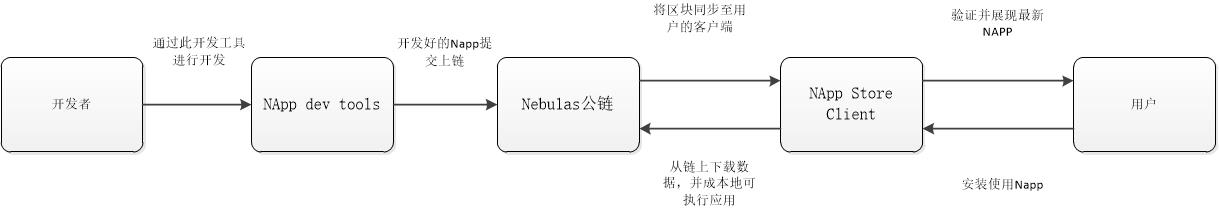
\includegraphics[width=.9\textwidth]{flow.jpg}
\caption{NApp Store 流程图}
\end{figure}

\subsection{NApp在链上的数据格式}
此处,我们给出NApp在链上的数据格式,以表明开发者需要提交哪些信息,并为后续的NApp Store Client的展示提供必要的数据。

我们使用protobuf的格式描述链上的数据结构。
\begin{verbatim}
message napp_dep_meta{
    string name = 1;
    uint64 version = 2;
};

message napp_data{
    string napp_name = 1;
    uint64 napp_version = 2;
    string napp_intro = 3;
    string napp_icon_url = 4;
    repeated napp_dep_meta napp_depends = 5;
    bytes napp_ir = 6;
};

\end{verbatim}
\noindent 其中,\texttt{napp\_name},\texttt{napp\_version},\texttt{napp\_intro},\texttt{napp\_icon\_url}的含义是明显的,需要注意的是\texttt{napp\_name}及\texttt{napp\_intro}皆有一定的长度限制。
\texttt{napp\_depends}定义了该NApp所依赖的库及版本号,\texttt{napp\_ir}为该NApp对应的LLVM IR。

另外,需要注意的是,由于一个transaction附带的binary data的长度通常有大小限制,因此,\texttt{napp\_data}的总长度不能超过对应的上限。目前,Nebulas主网对这一限制为128KB,这一限制可以进一步放松或解除。

\subsection{NApp能做什么?}
NApp并不是简单的智能合约或者简单的与智能合约的交互,NApp的能力很大程度上由其所依赖的库决定。最基础的部分,是一个NApp具有本地的与NAS账户、Nebulas主网及Nebulas主网之上的智能合约交互的能力;
更进一步的,NApp能够使用图形界面与用户进行交互、能够使用引擎创造更加本地化的应用体验。

举个例子,用户可以在NApp Store Client内安装一个书籍NApp,并在书籍NApp内完成支付、阅读、甚至评价等操作。
需要注意的是,其中的支付环节使用了书籍NApp与Nebulas交互的能力,阅读则使用了本地化的图形界面,最后的评价操作甚至涉及中心化的社交网络交互操作。
从这个例子中不难看出,NApp能够在使用区块链方面创造出流畅的用户体验。这将完全不同于现有的DApp需要使用额外的钱包或钱包插件的用户体验。

另外,从开发者的角度来看,开发NApp仅需要考虑本地化的开发及用户体验。这也有别于传统的DApp的开发,在DApp的开发中,由于智能合约不能提供本地化的交互体验,
因此,开发者需要通过前端(移动客户端或网页客户端)与智能合约进行交互,更复杂的,前端需要通过开发者自己架设的中心化服务器与区块链进行交互,这很大程度上增加了开发者的负担,同时也影响了用户体验。

\subsection{NApp与DApp的区别}
从概念上来说,NApp与DApp都包含了区块链交互的部分及用户交互的部分,其中区块链交互的部分通过智能合约,而在其他部分,这两者并不尽相同。

对于一个DApp,一般通过Web,或本地的客户端向用户提供交互接口,而Web或相应的客户端通过外部的钱包软件或插件与区块链进行交互,在一些情况下,Web或相应的客户端也可以通过中心化的服务器与区块链进行交互。
此时,由于缺乏统一的与区块链交互的方式,使得DApp在使用过程中,需要依赖外部的钱包软件或插件;更进一步地,Web、不同客户端之间的差异也使得区块链的使用难以有一致的开发或使用体验。

NApp则基于NApp dev tools包含的SDK与区块链进行交互,并使用其中的SDK构建图形化的用户交互界面,而进一步的流程及细节则由SDK提供保证,既保证了开发的简易性,又提供了体验的一致性。

另外,相对于DApp,NApp的一个重要能力是能够以去中心化的方式完成自动升级。对于使用了Web的DApp,可以通过在服务器中部署新的代码,而对于使用了客户端的用户,则依赖于用户的主动升级。


\section{NApp Store Client}
NApp Store Client是用户使用NApp的入口,安装在用户的终端设备\footnote{如用户的Mac,Windows及Linux设备,甚至iOS及Android设备,此外,我们应该优先考虑Mac设备}上,包括以下组件
\begin{itemize}
\item \textbf{P2P网络} --- P2P网络负责接入整个Nebulas主网的网络,同步Nebulas主网中的区块;
\item \textbf{区块验证} --- 负责对接收到的区块进行必要的验证,丢掉不必要的、无效的区块;
\item \textbf{NApp管理} --- 从经过验证的区块中读取\texttt{napp\_data},并存储在本地的数据库中,建立相关的索引信息;
\item \textbf{资产及私钥管理} --- 这不是NApp Store Client的主要功能,此功能仅仅是为了用户在使用NApp的过程中,能够进行必要的支付操作;
\item \textbf{NApp依赖库} --- 包含一个NApp运行所必要的程序库,如UI、发起交易等;
\item \textbf{UI交互} --- NApp Store Client将包含一个完整的、图形化的用户交互界面。
\end{itemize}

NApp Store Client从功能上来说包括三个部分,NApp的管理、NApp的安装及运行、资产及私钥管理。
\paragraph{NApp的管理}
NApp Store Client可以认为是Nebulas主网的一个轻节点,即,会同步所有的区块信息并进行必要的区块信息验证,但是不会成为出块或验证节点,亦不具备任何的挖矿功能。这一方面是因为用户的终端机性能较弱(包括硬件和网络),
另一方面,也因为在终端机上进行开销较大的出块或验证操作会影响用户体验。

NApp Store Client仅仅保存必要的NApp的信息,而不会保存所有的区块信息。在同步、验证完所有的区块信息后,NApp Store Client会提取其中的NApp信息,而抛弃区块内的其他信息。
这主要是因为区块数据过为庞大,在用户终端中保存如此规模的数据会极大的影响用户体验。

NApp Store Client会保存所有的NApp信息,包括同一个NApp的不同版本。这是为了让用户能够选择不同的版本。
\paragraph{NApp的安装及运行}
NApp Store Client会在UI中展示所有的NApp及NApp相关的信息,如NApp的图标、名称、描述及版本号。用户可以有选择安装指定的NApp。

NApp的安装过程实际上是使用LLVM相关工具将NApp相应的LLVM IR编译为本地代码,并与NApp依赖的库链接成本地的可执行文件的过程。相应的,NApp的运行实际上是用户直接运行生成的、本地的可执行文件。

\paragraph{资产及私钥管理}
为了提供本地化的支付体验,NApp Store Client需要管理一定的资产及相应的私钥。需要注意的是,NApp Store Client本身没有更多的资产或私钥管理的需求,更多的功能是仅仅是可选的,而不是必须的。
\section{NApp Dev Tools}

NApp dev tools供开发者使用,包括但不限于
\begin{itemize}
\item \textbf{NApp SDK}
\item \textbf{资产及公私钥管理}
\item \textbf{NApp开发及调试工具}
\item \textbf{NApp提交工具}
\end{itemize}


\section{几个问题}
NApp Store需要面临很多问题,此处仅讨论一些必要的权衡以及可能产生的影响。注意,以下所做的权衡都是根据目前的现状得出的,随着NApp Store的发展,这些权衡可能需要重新考虑。
\subsection{关于付费NApp}
目前,我们认为所有的NApp本身都是免费的,这很大程度上是因为使用付费的手段购买NApp较为复杂,而实现这一复杂的功能,即,实现付费NApp,并不能带来可预期的收益;
另一方面,开发者的收益可以通过NApp内的支付或者开发者激励协议(DIP)来保证。
\subsection{支付流程}
我们认为,每个NApp都需要一定的支付场景,因此,我们希望每个NApp的支付体验是一致的。为此,需要NApp Store Client提供统一的支付流程,以库的形式提供给NApp使用。

\subsection{NApp升级流程}
一个NApp实质上是一个具有一定标识的LLVM IR,且该LLVM IR是放在链上的,因此NApp的升级是通过NBRE的能力完成的。
\section{总结}

%\newpage
%\bibliography{reference}

%\newpage
%\begin{appendices}
%\end{appendices}

\end{document}
